\recipe{Ben's Gobi Manchurin}
\label{recipe:gobi_manchurin}
\makes{2 portions}
\worktime{\SI{30} \minute}
\totaltime{\SI{30} \minute}
\source{Ben Smith}


\begin{ingredients}

  \item  1 small head cauliflower (Broken into medium sized florets) 
  \item Oil for deep frying 
\ingroup{Batter}
  \item \SI{65}{\gram} all-purpose flour
  \item \SI{32}{\gram} cornflour
  \item \SI{1}{\teaspoon} Kashmiri red chili powder or paste
  \item \qty{0.25}{\teaspoon} ground black pepper 
  \item \SI{0.25}{\teaspoon} salt
  \item \SI{0.25}{\cup} water
\ingroup{Gobi Manchurian Sauce}
  \item \SI{1.5}{\tablespoon} oil
  \item \SI{1}{\tablespoon} garlic fine chopped 
  \item \SI{0.5}{\tablespoon} ginger fine chopped 
  \item 1 green chili chopped
  \item \SI{0.33}{\cup} onions
  \item \SI{0.25}{\cup} bell pepper
  \item \SI{1}{\tablespoon} soya sauce
  \item \SI{2}{\tablespoon} Red Chilli sauce  
  \item \SI{2}{\tablespoon} tomato ketchup 
  \item \SI{0.5}{\teaspoon} Kashmiri red chili powder
  \item \SI{0.5}{\tablespoon} apple cider vinegar
  \item \SI{1}{\teaspoon} sugar 
  \item salt as needed 
  \item \SI{3}{\tablespoon} water 
  \item \SI{0.5}{\teaspoon} black pepper crushed or ground 
  \item \SI{0.125}{\teaspoon}salt 
  \item 1 spring onion greens chopped for garnish

\end{ingredients}


\begin{method}
Preparation

Add cauli to slightly hot water. Rest for 5 mins, rinse with cold water then
drain.

Pat dry as moisture in the gobi will make it soft and not crisp. 

Heat up the oil for deep frying on a medium heat. 

Meanwhile make the batter by adding cornstarch, all-purpose flour, red
chilli powder, black pepper and salt to a mixing bowl.

Mix and add water little by little as needed and make a free flowing
batter. Add salt to taste.

Add the cauli florets to the batter (in batches), coat them well.
 
Fry Cauliflower

Check oil is hot enough by dropping a small amount of batter into the oil.
The batter has to sizzle and rise to the surface without browning.

Pick up each cauliflower floret with fingers \& gently drop them one by
one into the hot oil. Increase heat slightly as more gobi is added. Avoid
disturbing/stiring them for 1 to 2 minutes. 

Reduce the flame to medium and fry until the florets turn golden and
crisp. Keep stirring in between for even frying. Remove them from the
pan shaking gently to get rid of the excess oil. 

Transfer to a paper towel or a steel colander. Repeat steps 1-3 for the rest
of the cauli. Oil should not be smoking hot, before you fry the next batch. 

Make Gobi Manchurian

Prepare the sauce: Add soy sauce, red chili sauce, tomato ketchup, red
chilli paste, sugar and vinegar to a small bowl and keep this aside. 

Heat oil in a wide pan or wok. Add garlic, ginger and green chilies. Saute
for 2 minutes.

Add spring onion whites \& pepper. Saute them on a high for 2 mins.

Pour in the sauce and water. Mix well and cook stirring until the sauce
turns thick. Add black pepper and turn off the heat. 

Taste test and adjust the heat and salt levels to your taste. The sauce has
to be slightly tangy, sweet \& hot.

Allow the sauce to cool for 1 to 2 mins. Add the fried cauliflower and stir
gently to coat well with the manchurian sauce. 

Garnish gobi manchurian with spring onion greens. Serve immediately as
a appetizer or as a side with noodles or fried rice.
  
\end{method}


\begin{figure}[h]
  	\centering
  	
	\begin{tikzpicture}
  		% Save the image in a box to get its dimensions
  		\sbox0{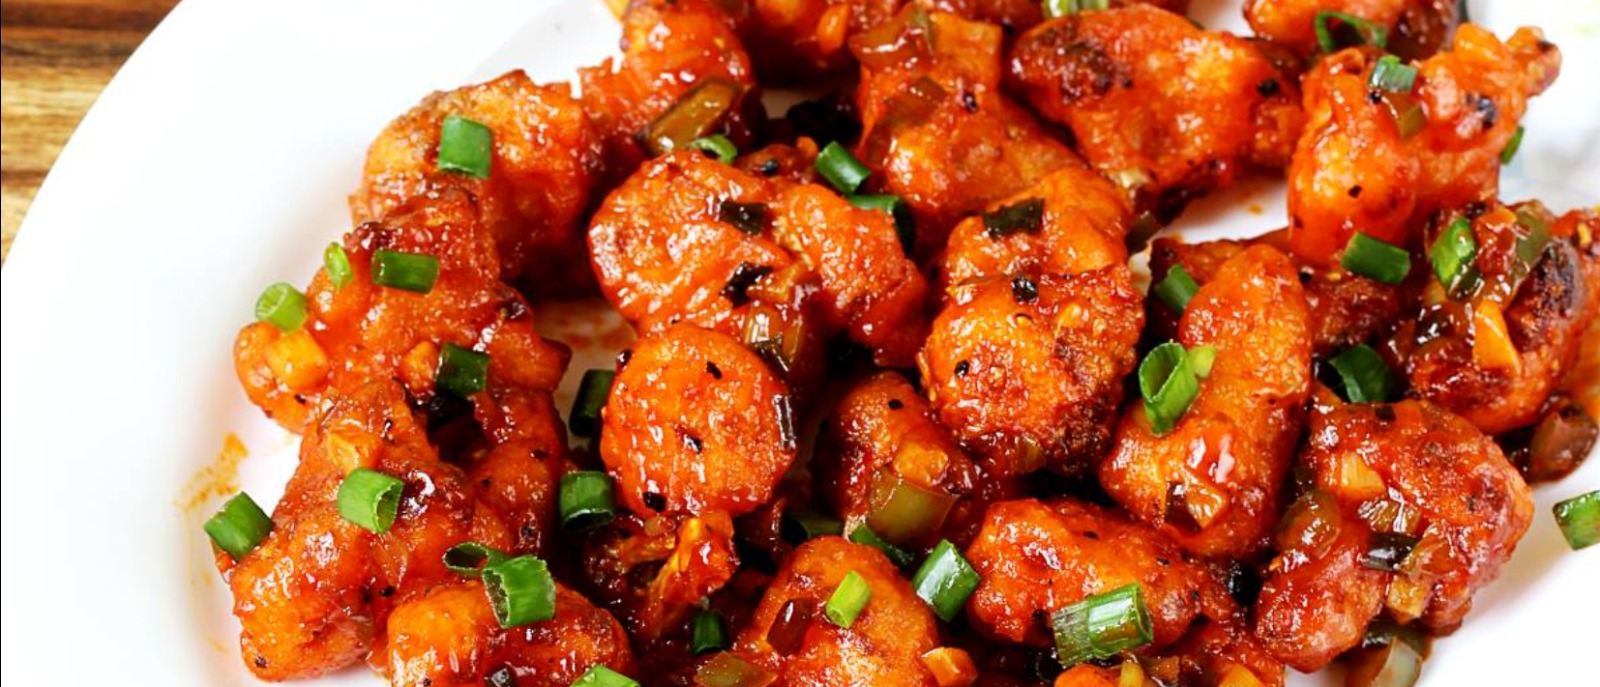
\includegraphics[width = \linewidth]{images/gobiManchurian.jpeg}}%
  
  		% Draw a clipping rectangle with rounded corners
  		\path[clip, rounded corners=0.5cm] (0,0) rectangle (\wd0,\ht0);
  
  		% Place the image inside the clipped area
  		\node[inner sep=0pt, outer sep=0pt, anchor=south west] at (0, 0) {\usebox0};
	\end{tikzpicture}

\end{figure}




